\documentclass[letterpaper, 12pt]{math}

\usepackage{amsmath}
\usepackage{amssymb}
\usepackage{geometry}
\usepackage{tikz}

\geometry{letterpaper, margin=0.5in}

\title{Linear Algebra: Homework 1}
\author{Alvin Lin}
\date{August 2016 - December 2016}

\begin{document}

\maketitle

\subsection*{Exercise 1}
Draw the following vectors in standard position in \( \R^{2} \):
\[
  a = \begin{bmatrix} 3 \\ 0 \end{bmatrix} \quad
  b = \begin{bmatrix} 2 \\ 3 \end{bmatrix} \quad
  c = \begin{bmatrix} -2 \\ 3 \end{bmatrix} \quad
  d = \begin{bmatrix} 3 \\ -2 \end{bmatrix}
\]
\begin{center}
  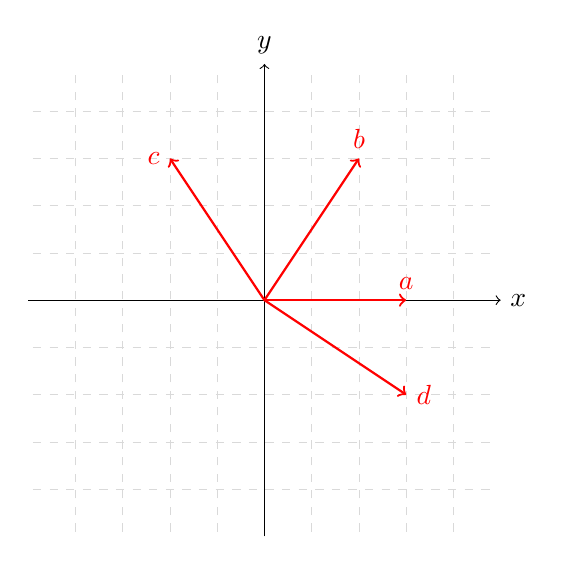
\begin{tikzpicture}[scale=0.6]
    \draw[help lines, color=gray!30, dashed] (-4.9,-4.9) grid (4.9,4.9);
    \draw[->] (-5,0)--(5,0) node[right] {\( x \)};
    \draw[->] (0,-5)--(0,5) node[above] {\( y \)};
    \draw[->,red,thick] (0,0)--(3,0) node[above] {\( a \)};
    \draw[->,red,thick] (0,0)--(2,3) node[above] {\( b \)};
    \draw[->,red,thick] (0,0)--(-2,3) node[left] {\( c \)};
    \draw[->,red,thick] (0,0)--(3,-2) node[right] {\( d \)};
  \end{tikzpicture}
\end{center}

\subsection*{Exercise 3}
Draw the following vectors in standard position in \( \R^{3} \):
\begin{flalign*}
  a &= [0,2,0] &\\
  b &= [3,2,1] \\
  c &= [1,-2,1] \\
  d &= [-1,-1,-2]
\end{flalign*}

\subsection*{Exercise 5}
For each of the following pairs of points, draw the vector \( \vec{AB} \). Then
compute and redraw \( \vec{AB} \) as a vector in standard position.
\[ A = (1,-1), B = (4,2) \]
\begin{center}
  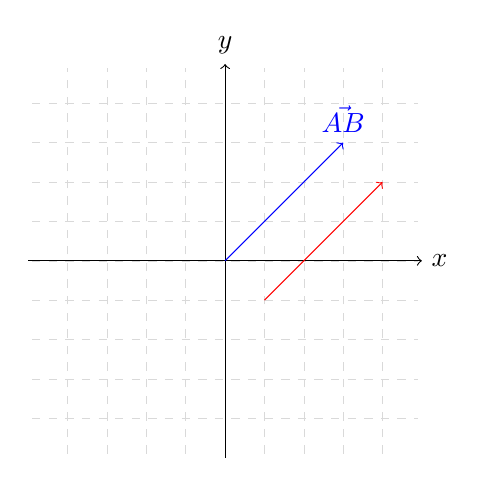
\begin{tikzpicture}[scale=0.5]
    \draw[help lines, color=gray!30, dashed] (-4.9,-4.9) grid (4.9,4.9);
    \draw[->] (-5,0)--(5,0) node[right] {\( x \)};
    \draw[->] (0,-5)--(0,5) node[above] {\( y \)};
    \draw[->,red] (1,-1)--(4,2);
    \draw[->,blue] (0,0)--(3,3) node[above] {\( \vec{AB} \)};
  \end{tikzpicture}
\end{center}
\[ A = (0,-2), B = (2,-1) \]
\begin{center}
  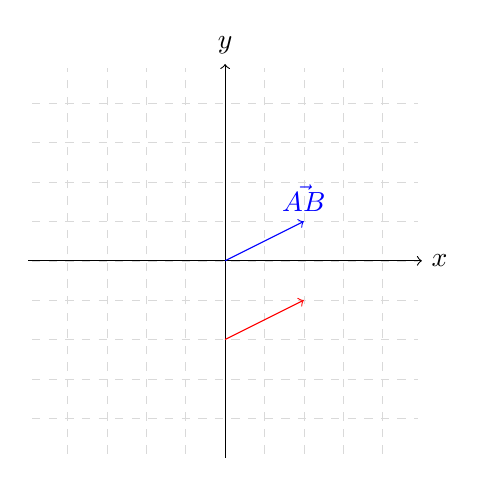
\begin{tikzpicture}[scale=0.5]
    \draw[help lines, color=gray!30, dashed] (-4.9,-4.9) grid (4.9,4.9);
    \draw[->] (-5,0)--(5,0) node[right] {\( x \)};
    \draw[->] (0,-5)--(0,5) node[above] {\( y \)};
    \draw[->,red] (0,-2)--(2,-1);
    \draw[->,blue] (0,0)--(2,1) node[above] {\( \vec{AB} \)};
  \end{tikzpicture}
\end{center}
\[ A = (2,\frac{3}{2}), B = (\frac{1}{2},3) \]
\begin{center}
  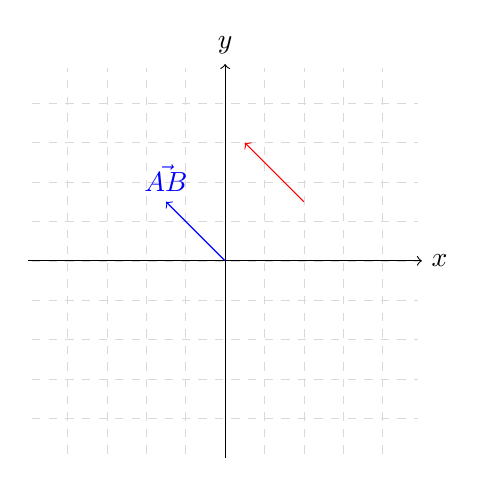
\begin{tikzpicture}[scale=0.5]
    \draw[help lines, color=gray!30, dashed] (-4.9,-4.9) grid (4.9,4.9);
    \draw[->] (-5,0)--(5,0) node[right] {\( x \)};
    \draw[->] (0,-5)--(0,5) node[above] {\( y \)};
    \draw[->,red] (2,1.5)--(0.5,3);
    \draw[->,blue] (0,0)--(-1.5,1.5) node[above] {\( \vec{AB} \)};
  \end{tikzpicture}
\end{center}
\[ A = (\frac{1}{3},\frac{1}{3}), B = (\frac{1}{6},\frac{1}{2}) \]
\begin{center}
  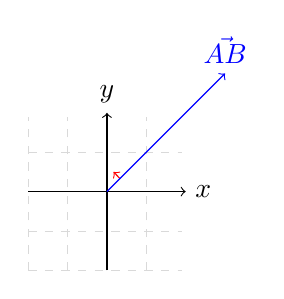
\begin{tikzpicture}[scale=0.5]
    \draw[help lines, color=gray!30, dashed] (-2,-2) grid (1.9,1.9);
    \draw[->] (-2,0)--(2,0) node[right] {\( x \)};
    \draw[->] (0,-2)--(0,2) node[above] {\( y \)};
    \draw[->,red] (0.33,0.33)--(0.166,0.5);
    \draw[->,blue] (0,0)--(3,3) node[above] {\( \vec{AB} \)};
  \end{tikzpicture}
\end{center}

\subsection*{Exercise 7}
Compute the indicated vectors from Exercise 1 and show how the results can be
obtained geometrically.
\begin{flalign*}
  a+b &= \langle3,0\rangle+\langle2,3\rangle &\\
  &= \langle5,3\rangle
\end{flalign*}

\subsection*{Exercise 9}
Compute the indicated vectors from Exercise 1 and show how the results can be
obtained geometrically.
\begin{flalign*}
  d-c &= \langle3,-2\rangle-\langle-2,3\rangle &\\
  &= \langle5,-5\rangle
\end{flalign*}

\subsection*{Exercise 11}
Compute the indicated vectors from Exercise 3.
\begin{align*}
  2a+3c &= 2\langle0,2,0\rangle+2\langle1,-2,1\rangle \\
  &= \langle0,4,0\rangle+\langle2,-4,2\rangle \\
  &= \langle2,0,2\rangle
\end{align*}

\subsection*{Exercise 13}
Find the components of the vectors \( u,v,u+v,u-v \) where \( u \) and \( v \)
are as shown in Figure 1.23.
\begin{align*}
  u &= \langle\cos(60),\sin(60)\rangle =
    \langle\frac{1}{2},\frac{\sqrt{3}}{2}\rangle \\
  v &= \langle\cos(30),\sin(30)\rangle =
    \langle\frac{\sqrt{3}}{2},\frac{1}{2}\rangle \\
  u+v &= \langle\frac{1+\sqrt{3}}{2},\frac{1+\sqrt{3}}{2}\rangle \\
  u-v &= \langle\frac{1-\sqrt{3}}{2},\frac{\sqrt{3}-1}{2}\rangle
\end{align*}

\subsection*{Exercise 15}
\begin{align*}
  2(a-3b)+3(2b+a) &= 2a-6b+6b+3a \\
  &= 5a
\end{align*}

\subsection*{Exercise 17}
\begin{align*}
  x-a &= 2(x-2a) \\
  x-a &= 2x-4a \\
  x &= 2x-4a+a \\
  -x &= -3a \\
  x &= 3a
\end{align*}

\subsection*{Exercise 24}
Give algebraic proofs of properties (d) through (g) of Theorem 1.1: \\
Proof of (d):
\begin{align*}
  \vec{u}+(-\vec{u}) &= \langle u_{1},u_{2},\dots,u_{n}\rangle+
    \langle-u_{1},-u_{2},\dots,-u_{n}\rangle \\
  &= \langle u_{1}-u_{1},u_{2}-u_{2},\dots,u_{n}-u_{n}\rangle \\
  &= \langle0,0,\dots,0\rangle = \vec{0}
\end{align*}
Proof of (e):
\begin{align*}
  c(\vec{u}+\vec{v}) &= c(\langle u_{1},u_{2},\dots,u_{n}\rangle+
    \langle v_{1},v_{2},\dots,v_{n}\rangle) \\
  &= c(\langle u_{1}+v_{1},u_{2}+v_{2},\dots,u_{n}+v_{n}\rangle) \\
  &= \langle c(u_{1}+v_{1}),c(u_{2}+v_{2}),\dots,c(u_{n}+v_{n})\rangle \\
  &= \langle cu_{1}+cv_{1},cu_{2}+cv_{2},\dots,cu_{n}+cv_{n}\rangle \\
  &= \langle cu_{1},cu_{2},\dots,cu_{n}\rangle+
    \langle cv_{1},cv_{2},\dots,cv_{n}\rangle \\
  &= c\langle u_{1},u_{2},\dots,u_{n}\rangle+
    c\langle v_{1},v_{2},\dots,v_{n}\rangle \\
  &= c\vec{u}+c\vec{v}
\end{align*}
Proof of (f):
\begin{align*}
  (c+d)\vec{u} &= (c+d)\langle u_{1},\dots,u_{n}\rangle \\
  &= \langle(c+d)u_{1},\dots,(c+d)u_{n}\rangle \\
  &= \langle cu_{1}+du_{1},\dots,cu_{n}+du_{n}\rangle \\
  &= \langle cu_{1},\dots,cu_{n}\rangle+\langle du_{1},\dots,du_{n}\rangle \\
  &= c\vec{u}+d\vec{u}
\end{align*}
Proof of (g):
\begin{align*}
  c(d\vec{u}) &= (c)\langle du_{1},\dots,du_{n}\rangle \\
  &= (c)(d)\langle u_{1},\dots,u_{n}\rangle \\
  &= (cd)\langle u_{1},\dots,u_{n}\rangle \\
  &= (cd)\vec{u}
\end{align*}

\begin{center}
  If you have any questions, comments, or concerns, please contact me at
  alvin@omgimanerd.tech
\end{center}

\end{document}
